
\documentclass[11pt,twocolumn]{article}
\usepackage{lmodern,setspace,amsmath,amssymb,amsfonts,amsthm,graphicx,multicol,grffile,float}
\usepackage{authblk,url,csvsimple,cuted,dblfloatfix,stfloats,parskip}
\usepackage[a4paper, top=0.9in, bottom=1.05in, left=1.01in, right=1.01in]{geometry}
\usepackage[polish]{babel}
\usepackage[utf8]{inputenc}
\usepackage[T1]{fontenc}
\usepackage{algorithm2e}
\title{Optymalizacja kombinatoryczna - Sprawozdanie 2. \\ Zastosowanie funkcji ciągłych dla problemu job-shop}
\author{Dariusz Max Adamski 136674, Daniel Cieśliński 136695}
\affil{\{dariusz.adamski,daniel.cieslinski\}@student.put.poznan.pl}
\date{Data oddania:}

\begin{document}

\maketitle


\section*{Wstęp}

W tym sprawozdaniu przedstawione zostanie autorskie podejście do problemu szeregowania zadań (job-shop) \cite{ortools}.
Porównana będzie jakość rozwiązań w odniesieniu do ograniczenia dolnego instancji.
Omawiany w tym sprawozdaniu algorytm, pozwala na rozwiązanie problemu szeregowania zadań, bez reprezentacji grafowej owego problemu.


\section{Opis problemu}

Dla każdej instancji problemu szeregowania zadań,
zdefiniowane jest $\mathcal{J}$ zadań (jobs) oraz $\mathcal{M}$ maszyn.
Każde zadanie składa się z $\mathcal{M}$ operacji (tasks),
których kolejność jest znacząca.
$j$-ta operacja $i$-tego zadania musi być wykonywana na określonej maszynie $m_{ij}$,
przez określony czas $t_{ij}$.

Rozwiązanie uzyskujemy decydując o kolejnościach i
czasach startowych wykonywania operacji na każdej maszynie.

Makespan to czas w którym zostało zakończone ostatnie zadanie.
Celem programu jest minimalizacja tego kryterium.

\section{Ogólny schemat działania algorytmu}
Algorytm składa się z trzech głównych bloków, następujący pseudokod opisuję procedurę ustalania kolejności przypisania wierzchołków do harmonogramu. Pierwszy blok jest opisany, przez poniższy pseudokod.
\begin{algorithm}
\KwData{$jobs$ such that each job consist of M tasks on M different machines.}
\KwResult{$Alignment$ Order in which tasks are going to be aligned on schedule}
\DontPrintSemicolon
$iter \longleftarrow 0$\\
$alignment \longleftarrow \emptyset$\\
key=lambda x,y :x.func[iter] > y.func[iter] \\
\Begin{

\For{i < number\_of\_jobs}{
    $poss\_choices \longleftarrow \emptyset$\\
    \For{job in jobs}{
        \If{not(job.finished)}{
            poss\_choices.add(job[job.next])
        }
    }
}
sort(poss\_choices, key=key)

\For{k < poss\_choices.size()}{
    \If{rand(0,1) < dropout}{
        continue
    }
    t = poss\choices[k]\\
    alignment.add(t)\\
    iter += 1\\
    jobs[t.job].next += 1\\
    \If{jobs[t.job].next == job.tasks.size()}{
        jobs[t.job].finished = true
    }
    if task was't selected due to dropout\\
    select random from poss\_choices
    }
}
    % \caption{Wybór wierzchołków na podstawie wartości funkcji X}
\end{algorithm}
\\
Po tym jak algorytm wybierze zadania bazując na wartości funkcji X, zajmuje się dopasowaniem kolejno wybranych zadań, tak aby zminimalizować czas oczekiwania maszyny na kolejne zadanie.
Dla przykładu rozważmy następujące zadanie:\\

$job \longleftarrow 0$ \\
$order \longleftarrow 1$ \\
$time \longleftarrow 3$ \\
$machine \longleftarrow 0$ \\
\\
W tablicy $machine\_times$ zapisane są przedziały czasowe w których maszyna  jest zajęta. Przedziały są prawostronnie otwarte, a lewostronnie domknięte. 

$machine\_times \longleftarrow [\{0,2\}, \{6,7\}]$ 

Program iteruje przez przedziały w maszynie i sprawdza, czy możliwe jest dopasowanie zadania, tak aby zminimalizować span. 
Jest to wykonywane przez sprawdzenie, czy istnieje w maszynie luka, która zmieści dane zadanie, biorąć pod uwagę minimalny czas w którym zadanie może rozpocząć pracę. Przez minimalny czas rozpoczęcia zadania rozumiemy, czas w którym kończy się, poprzednie zadanie tej samej pracy.

Na potrzeby demonstracji przyjmyjmy, że zadanie 0 pracy 0, kończy działanie w kwancie czasu 2, zatem od kwantu czasu 3 kolejne zadanie może zacząć być wykonywane. 

Wynikiem działania procedury, dla tego zadania  będzie następująca wartość zmiennych:


$machine\_times \longleftarrow [\{0,2\},\{3,6\},\{6,7\}]$ \\
$out \longleftarrow 3$ \\

Zmienna $out$ ma wartość kwantu czasu w której zadanie rozpocznie być przetwarzane przez maszynę.


Kolejny zadaniem programu jest propagacja wsteczna, która została opisana w sekcji $Funkcja  X$

\section{Funkcja X}
Funkcja X dana jest następującym wzorem:
$$f(x,p) = l\bigg( x - p - \sqrt{\frac{2}{-l}}\bigg)\bigg(x - p + \sqrt{\frac{2}{-l}}\bigg)$$

gdzie:\\
$l=ln(b)$, natomiast $b$, to wspołczynnik propagacji i $b \in (0,1)$ \\
p - indeks, w którym zadanie zostało dodane do listy alignment w pierwszej procedurze

\subsection{Propagacja wsteczna}
Kiedy zakończone zostaną wszystkie poprzednie procedury dla danej iteracji algorytmu, dochodzi do progacji wstecznej. W tej części programu dla każdego zadania wykonywana jest następująca procedura:

\begin{algorithm}
\Begin{

\For{i < func.size()}{
    func[i] *= decr\_param \\
}

\For{i in (i\_min, i\_max)}{
    val = $\frac{f(x,p) + func[i]}{2}$\\
    \If{!better}{
        val*=bad\_param\\    
        }
    func[i] = val\\
    }
}
\end{algorithm}

gdzie:\\
$p$ -indeks, w którym zadanie zostało dodane do listy alignment w pierwszej procedurze\\
$bad\_param$ - wartość razy jaką mnożymy, kiedy makespan przetwarzanego harmonogramu, nie był lepszy najlepszego wykrytego\\
$better$ - Czy przebieg był lepszy, czyli, czy dany przebieg miał lepszy makespan\\
$decr\_param$ - parametr, razy jaki mnożymy poprzednie wartości funkcji. Zastosowanie parametrów poniżej.

\subsection{Charakterystyka funkcji}

Poniższy wykres jest wykresem funkcji $f(x,p)$ dla $x,p \in [0,100]$
przy stałej wartości parametru propagacji.
Funkcja przyjmuje argumenty mniejsze od zera, jednak w implementacji bierzemy pod uwagę tylko wartości większe od zera.

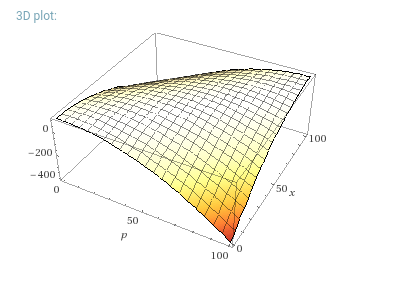
\includegraphics[width=\linewidth]{0999.png}

Parametr propagacji określa ile sąsiednich indeksów będzie afektowanych, przez poprawność danego uszeregowania. Ilustrują to wykresy poniżej. Pierwszy wykres ilustruje funkcję z parametrem propagacji równym $0.8$, natomiast drugi z parametrem równym $0.999$

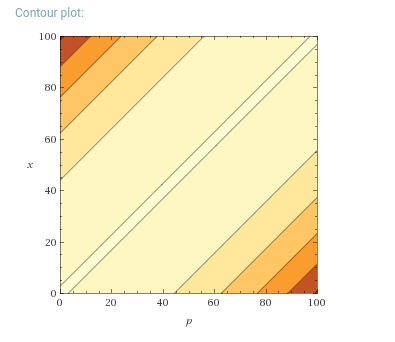
\includegraphics[width=\linewidth]{08plain.png}
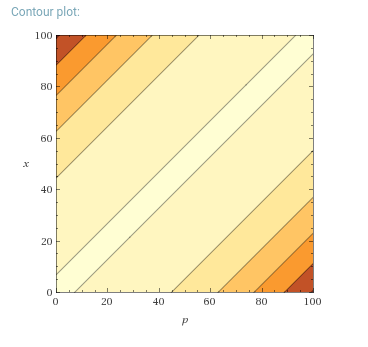
\includegraphics[width=\linewidth]{0999plain.png}

\section{Pomiary}

\subsection{Metodologia}

Instancje na których program był testowany to ,,tai'', ,,yn'', ,,fs'',
,,abz'', ,,ft'', ,,la'', ,,orb'', ,,swv'' i ,,dmu''.
Lącznie użyto 245 instancji problemu,
czyli wszystkich dostarczonych do zadania,
oraz instancje Demirkola \cite{bound}.

Program został przetestowany pod kątem poprawności,
na wszystkich instancjach,
przy użyciu sprawdzarki dostarczonej do zadania.

\subsection{Czas}

Na załączonym wykresie(pic 1), przedstawione zostały czasy rozwiązywania zadania przy stałej określonej na 10 tyś iteracji.
Pomiary były wykonywane przy kolejno ustawionych parametrach:
$dropout \longleftarrow 0.05$ \\
$propagation\_param \longleftarrow 0.95$ \\
$decr\_param \longleftarrow 0.95$ \\
$bad\_param \longleftarrow 0.3$ \\

% \begin{figure}[h!]
% 	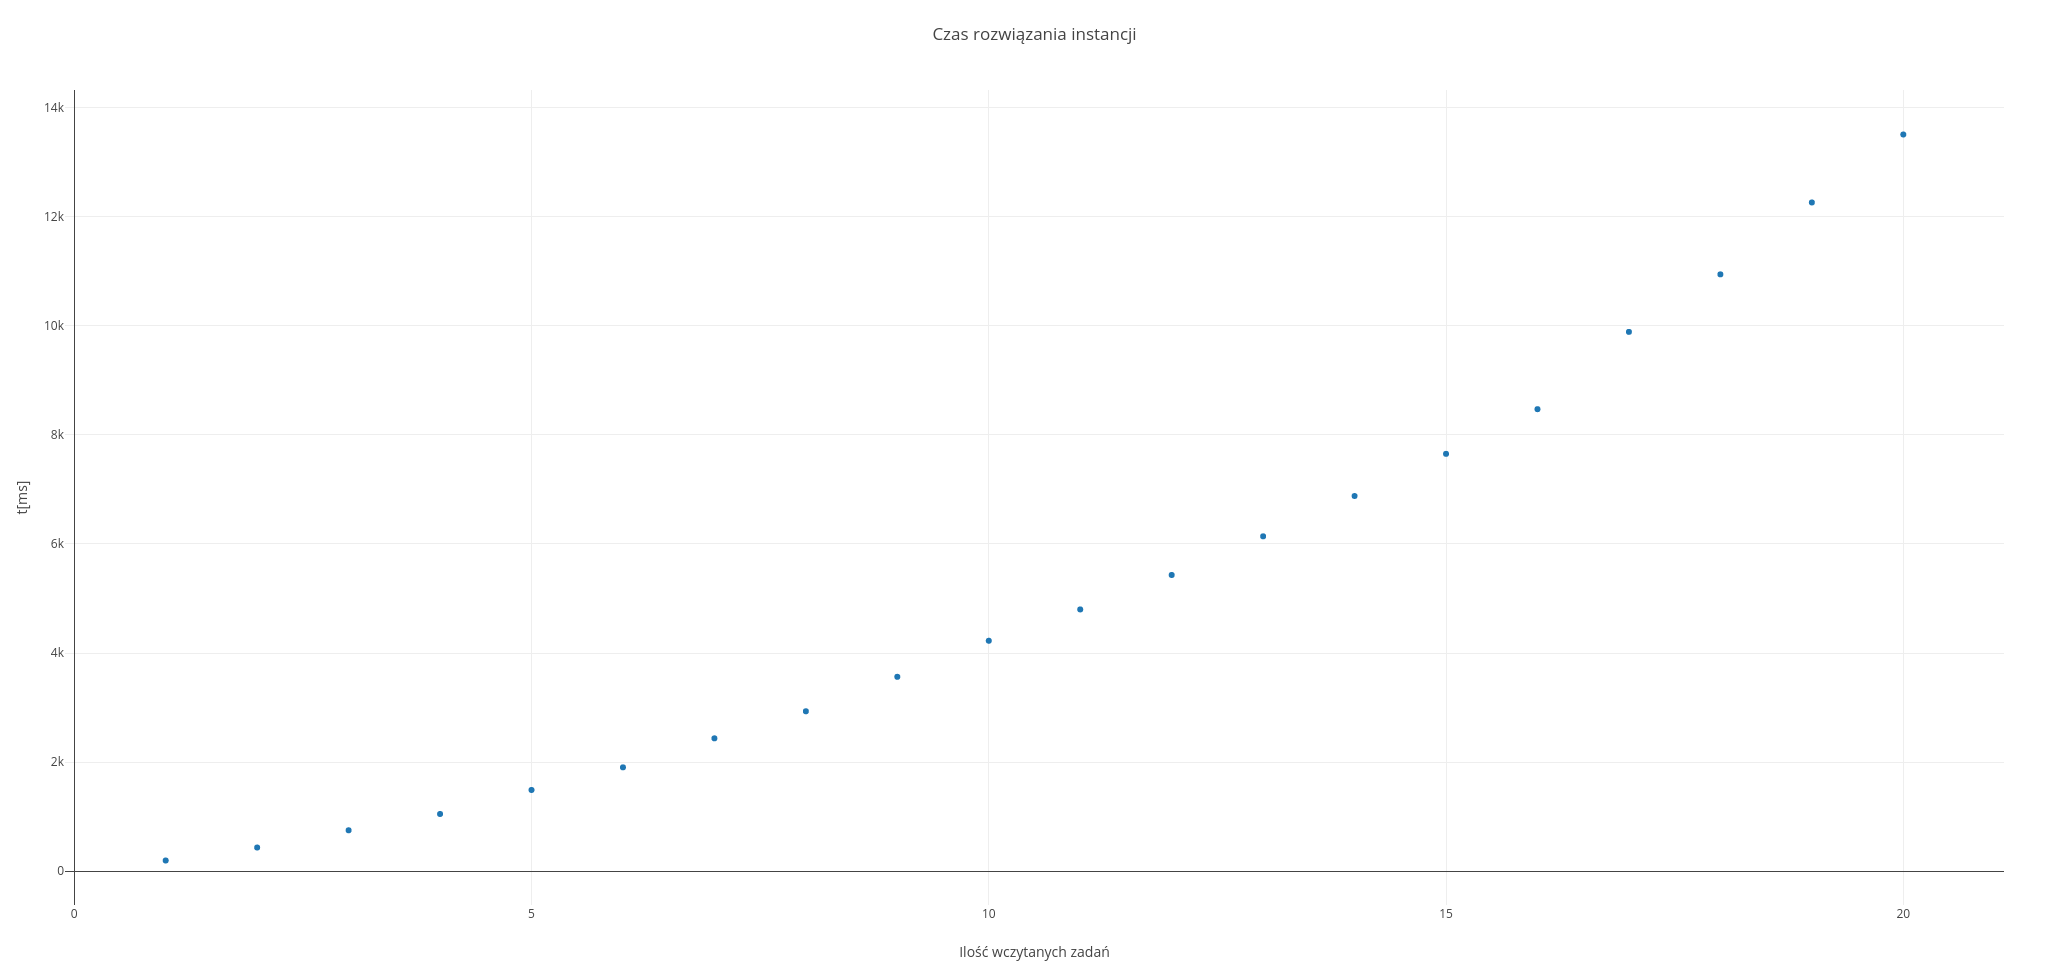
\includegraphics[width=\linewidth]{2018-12-07_08-21.png}
% 	\caption{Czas wykonywania dla instancji tai25, przy 10 tyś iteracji,
%         w zależności od ilości zadań.
%         Naniesiona linia trendu.
%         \label{tai_czas}}
% \end{figure}

\subsection{Porównanie jakości}

Aby ocenić jakość rozwiązań, w kolumnie ,,error'' tabeli \ref{tab1}
został obliczony błąd bezwględny w odniesieniu do ograniczenia dolnego,
według poniższego wzoru.
Alternatywnie można bezpośrednio porównać wartość ograniczenia dolnego/górnego
i makespan otrzymanego rozwiązania.

$$ error = \frac{|span - lb|}{lb} \cdot 100\% $$

Wyniki dla instancji Tailarda zostały przedstawione w tablicy numer 1.


\begin{table*}[b]
\centering
\begin{tabular}{l|rrrrrrrr}
    & $\mathcal{J}$ & $\mathcal{M}$ & lb  & ub   & span & x\_error & gr\_error  \\ \hline
    tai20 & 20  & 15 & 1348 & 1348 & 1801 & 33\% & 49\%\\
    tai21 & 20  & 20 & 1642 & 1642 & 2072 & 26\% & 34\%\\
    tai22 & 20  & 20 & 1561 & 1600 & 2101 & 34\% & 40\%\\
    tai23 & 20  & 20 & 1518 & 1557 & 2021 & 31\% & 49\%\\
    tai24 & 20  & 20 & 1644 & 1644 & 2126 & 29\% & 33\%\\
    tai25 & 20  & 20 & 1558 & 1595 & 2094 & 34\% & 38\%\\
\end{tabular}
\caption{Parametry instancji i jakość rozwiązania, algorytm był wykonywany z ograniczeniem minuty działania.}
\label{tab1}
\end{table*}


\section{Wnioski}

Zaprezentowany w tym sprawozdaniu algorytm, jest dowodem na to, że możliwe jest rozwiązanie problemu szeregowania zadań, przy użyciu funkcji ciągłych.
Pomysł na zaimplementowanie algorytmu łaczącego w sobie funkcje ciągłe i metodę monte-carlo, powstał niedawno i zdecydowanie wymaga jeszcze wiele pracy nad tym aby mogł konkurować z takimi heurystykami jak algorytm genetyczny, czy mrówkowy.


\newpage

\begin{thebibliography}{9}

\bibitem{ortools}
    \textit{The Job Shop Problem},
    \url{https://developers.google.com/optimization/scheduling/job_shop}

\bibitem{tai}
    \textit{Instancje Taillarda},
    \url{http://mistic.heig-vd.ch/taillard/problemes.dir/ordonnancement.dir/ordonnancement.html}

\bibitem{dem}
    \textit{Instancje Demirkola},
    \url{http://optimizizer.com/DMU.php}

\bibitem{bound}
    \textit{Ograniczenia dolne i górne instancji; Instancje Demirkola},
    \url{http://optimizizer.com/TA.php}

\end{thebibliography}

\end{document}

